\chapter{Verifica e validazione}
\label{cap:verifica-validazione}

\intro{In questo capitolo verranno descritte le attività di verifica e
    validazione del prodotto. In particolare verranno descritti i test di unità e di
    sistema, i risultati ottenuti ed eventuali migliorie future da applicare al
    prodotto.}

\section{Test di unità}

Uno dei requisiti fondamentali da soddisfare durante il progetto di stage è
quello riguardante la scrittura di test durante lo sviluppo del codice. In
questa sezione verranno descritti i test di unità, effettuati al fine di
verificare che le singole componenti del sistema funzionassero nella maniera prevista. \\
All'interno del codice, sia nei test, sia nel codice effettivo, sono state
inserite delle variabili d'ambiente che permettono di sostituire il percorso
legato ai profili colore utilizzati: così facendo si ha la possibilità di
eseguire i test anche in locale, senza dover necessariamente effettuare il
\emph{deploy} per verificare che tutto funzioni correttamente.\\
Ogni test di unità è contraddistinto da un codice identificativo, che segue la
seguente nomenclatura: \\
\begin{center}
    \textbf{TU[Codice]}
\end{center}
dove:
\begin{itemize}
    \item \textbf{TU:} definisce che il test è di unità;
    \item \textbf{Codice:} definisce il numero progressivo che contraddistingue il test.
\end{itemize}

Ad ogni test viene assegnato un esito, che può essere di due tipi:
\begin{itemize}
    \item \textbf{S:} il test è stato superato con successo;
    \item \textbf{NS:} il test non è stato superato.
\end{itemize}

Le seguenti tabelle \ref{tab:test-conversioni} e \ref{tab:test-dao} riportano la
lista dei test effettuati per le componenti del sistema, nello specifico quelle
riguardanti le conversioni e quelle riguardanti i \emph{DAO}.
\begin{table}[H]
    \caption{Tabella di tracciamento dei test di unità riguardanti le varie conversioni}
    \label{tab:test-conversioni}
    \centering
    \begin{tabularx}{\textwidth}{|c|c|X|c|}
        \hline
        \textbf{Codice}                  & \textbf{Oggetto} & \textbf{Descrizione}                                                                                                                                                                             & \textbf{Esito} \\
        \hline
        \verb|TU1|                       & VipsConversion   & Verifica del corretto funzionamento della conversione via libreria \emph{vips}, controllando che venisse impostata la risoluzione, il profilo colore, la qualità e il formato desiderati         & S              \\
        \hline
        \verb|TU2|                       & PSDConversion    & Verifica del corretto funzionamento
        della conversione via libreria \emph{go-psd}, controllando che venisse
        impostata la risoluzione desiderata senza
        alterare il rapporto prospettico & S                                                                                                                                                                                                                                    \\
        \hline
        \verb|TU3|                       & EPSConversion    & Verifica del corretto funzionamento della conversione via programma \emph{GhostScript}, controllando che venisse impostata la risoluzione desiderata                                             & S              \\
        \hline
        \verb|TU4|                       & RAWConversion    & Verifica del corretto funzionamento della conversione via programma \emph{Darktable}, controllando che venissero impostate la risoluzione, il profilo colore, la qualità e il formato desiderati & S              \\
        \hline
    \end{tabularx}
\end{table}

\begin{table}[H]
    \caption{Tabella di tracciamento dei test di unità riguardanti i \emph{DAO}}
    \label{tab:test-dao}
    \begin{tabularx}{\textwidth}{|c|c|X|c|}
        \hline
        \textbf{Codice}                                          &
        \textbf{Oggetto}                                         & \textbf{Descrizione }  & \textbf{Esito} \\
        \hline
        \verb|TU5|                                               & ClientConfigurationDAO & Verifica del
        corretto funzionamento del \emph{DAO} che ritorna la configurazione del
        cliente specificato                                      & S                                       \\
        \hline
        \verb|TU6|                                               & ConversionsBucketDAO   & Verifica del
        corretto funzionamento del \emph{DAO} che si occupa di effettuare il
        caricamento e il salvataggio dei file su \emph{S3}       & S                                       \\
        \hline
        \verb|TU7|                                               & ImageConversionJobsDAO & Verifica del
        corretto funzionamento del \emph{DAO} che si occupa di inserire ed
        effettuare l'aggiornamento dei \emph{job} di conversione & S                                       \\
        \hline
    \end{tabularx}
\end{table}

I test effettuati sono stati utili per mostrare lacune ed errori nel codice
scritto. Il codice delle funzioni testate non ha funzionato al primo tentativo,
ed è stato necessario riscrivere più volte le funzioni per ottenere il risultato
desiderato. \\
La scrittura dei test, in generale, è risultata semplice ed intuitiva: ho
utilizzato anche una caratteristica del linguaggio \emph{Go}, ossia i test
\emph{table-driven}: è possibile specificare una tabella di test per eseguire
più volte una stessa porzione di codice, con input differenti. Questo è
risultato molto utile per testare più agevolmente le multiple combinazioni di
conversioni possibili.

\section{Test di sistema}

In questa sezione vengono descritti i test di sistema effettuati sul progetto di
stage. Questi test hanno lo scopo di verificare il corretto funzionamento del
codice con tutti i formati di immagine supportati e con diverse configurazioni
per singolo cliente. Durante questo test viene verificato anche se i \emph{DAO}
funzionano correttamente, in quanto è stato replicato il funzionamento completo
del servizio. \\
Per effettuare la fase di test in locale, sono state necessarie diverse
componenti e software aggiuntivi, che ora andrò ad elencare:
\begin{itemize}
    \item \textbf{Immagini di test:} queste immagini venivano recuperate da una
          cartella denominata \emph{test-images}, in cui era presente un'immagine per
          ogni formato supportato e previsto dai requisiti funzionali;
    \item \textbf{Localstack:} è un \emph{framework} che permette di emulare
          alcuni servizi \emph{AWS} in locale, tra cui \emph{S3}. Questo servizio viene lanciato da uno script
          \glsfirstoccur\gls{bash}, che si occupa di creare i due \emph{bucket}
          necessari per l'\emph{upload} e il \emph{download} delle immagini; \cite{localstack}
    \item \textbf{Docker e docker-compose:} sono due strumenti che hanno
          permesso di creare in modo semplice e veloce un \emph{container} in cui
          creare due istanze di \emph{DynamoDB}, al fine di ricreare le tabelle della
          configurazione e dei \emph{job} di conversione. I database vengono creati a
          grazie ad un comando \emph{bash} che si occupa di lanciare il
          \emph{container} e creare le risorse seguendo il modello specificato nel
          file di infrastruttura del codice. Con \emph{Docker} è stato creato
          anche un \emph{container} su cui viene lanciata la \emph{Lambda}
          direttamente da riga di comando, solo dopo avere inserito le
          credenziali di accesso all'ambiente \emph{sandbox};
    \item \textbf{File JSON di configurazione:} è stato creato un file di tipo
          \emph{JSON} in cui sono state contenute alcune configurazioni di test per il
          cliente \emph{test-client}. Nello specifico le configurazioni sono state le
          seguenti:
          \begin{itemize}
              \item \textbf{Configurazione "ORIGINAL":} larghezza impostata a $0$,
                    altezza impostata a $0$, qualità impostata a $100$. Si è deciso di
                    utilizzare come valore sentinella lo $0$, così da poter verificare che
                    venissero utilizzate le dimensioni originali dell'immagine in ingresso
                    per la conversione;
              \item \textbf{Confiurazione "4K":} larghezza impostata a $3840$, altezza
                    impostata a $2160$, qualità impostata a $100$;
              \item \textbf{Configurazione "2K":} larghezza impostata a $2560$, altezza
                    impostata a $1440$, qualità impostata a $100$;
              \item \textbf{Configurazione "FULLHD":} larghezza impostata a $1920$,
                    altezza impostata a $1080$, qualità impostata a $100$;
              \item \textbf{Configurazione "HD":} larghezza impostata a $1280$, altezza
                    impostata a $720$, qualità impostata a $100$;
          \end{itemize}
\end{itemize}

Ogni test di sistema è contraddistinto da un codice identificativo, che segue la
seguente nomenclatura: \\
\begin{center}
    \textbf{TS[Codice]}
\end{center}
dove:
\begin{itemize}
    \item \textbf{TS:} definisce che il test è di sistema;
    \item \textbf{Codice:} definisce il numero progressivo che contraddistingue il test.
\end{itemize}

Di seguito viene riportata la tabella \ref{tab:test-sistema} che riporta i test
di sistema effettuati sul progetto di stage.

\begin{table}[H]
    \caption{Tabella di tracciamento dei test di sistema}
    \label{tab:test-sistema}
    \begin{tabularx}{\textwidth}{|c|c|X|c|}
        \hline
        \textbf{Codice}                                      & \textbf{Oggetto} & \textbf{Descrizione}                           & \textbf{Esito} \\
        \hline
        \verb|TS1|                                           & Conversione      & Verifica del corretto funzionamento
        del servizio di conversione per ogni immagine, verificando che la stessa
        venga convertita correttamente, seguendo la configurazione recuperata e
        impedendo la conversione in caso di \emph{upscaling} & S
        \\
        \hline
        \verb|TS2|                                           & DAO              & Verifica del corretto funzionamento di tutti i
        DAO, controllando che venga eseguito il recupero della configurazione della
        conversione, che venga effettuato il \emph{download} dell'immagine da
        convertire e che venga caricata nel \emph{bucket} di destinazione al termine
                                                             & S
        \\
        \hline
    \end{tabularx}
\end{table}

\section{Documentazione}

Un obiettivo obbligatorio previsto dal progetto di stage è stato quello di redigere la
documentazione sul progetto svolto, di tipo funzionale e tecnico. La prima delle
due è stata realizzata per descrivere il funzionamento del servizio a tutto il
team \emph{Contenuti}, fornendo informazioni utili a seguire il flusso della
conversione e per fornire una guida su come viene utilizzato il servizio. La documentazione tecnica invece pone l'attenzione sui dettagli
implementativi del codice ed è stata realizzata per fornire informazioni
riguardanti il codice e le tecnologie utilizzate per chi lavora nel lato \emph{back-end} del team: così facendo chiunque si troverà a
lavorare sul progetto potrà farlo in autonomia.\\
La documentazione è stata validata dal tutor aziendale, che ha accompagnato il
processo di stesura fornendo \emph{feedback} sulle parti da migliorare e
approfondire, man mano che venivano implementate nuove funzionalità. \\
Di seguito vengono descritte nel dettaglio le due tipologie di documentazione:
\begin{itemize}
    \item \textbf{Documentazione funzionale:} la documentazione funzionale è
          stata scritta in modo da essere comprensibile anche a chi non ha esperienza
          tecnica sul progetto. Viene infatti fornita una panoramica generale del
          servizio, elencandone le funzionalità ad alto livello ed il flusso di
          conversione seguito.
    \item \textbf{Documentazione tecnica:} la documentazione tecnica presenta
          tutte le informazioni necessarie per poter lavorare sul progetto in
          maniera autonoma, fornendo le informazioni riguardanti i comandi per
          installare gli applicativi e le librerie necessarie al corretto
          funzionamento del servizio. Sono presenti anche i comandi per
          effettuare la validazione dello \emph{stack} di risorse definito e per
          effettuare il \emph{deploy}. \\
          Vengono elencati i comandi per preparare l'ambiente di test in
          locale, fornendo una guida su come eseguire i \emph{container} che
          raccolgono i servizi \emph{AWS} emulati, e vengono fornite
          informazioni su come poter eseguire una dimostrazione del servizio,
          lanciando la \emph{Lambda} da riga di comando con una serie di
          conversioni di test.
\end{itemize}

Entrambe le documentazioni sono state inserite nel file \emph{README} presente
all'interno del progetto, così da essere sempre disponibile durante il lavoro
sul codice.

\section{Collaudo}

Durante il periodo di stage, sono stati previsti dei momenti di verifica
informale con il tutor aziendale, al fine di mostrare i progressi ottenuti sul
progetto e per ricevere \emph{feedback} sulle funzionalità implementate. Durante
le fasi di sviluppo sono state effettuate delle \glsfirstoccur\gls{pull-request}
su \emph{CodeCommit}, così da poter mantenere una versione stabile del progetto
nel ramo \emph{main} del repository ed avere una versione dove poter integrare
tutte le nuove funzionalità nel ramo \emph{dev}. Le funzionalità del ramo
\emph{dev} considerate stabili dovevano essere sottoposte al processo di
\glsfirstoccur\gls{code-review} da parte del tutor aziendale, al fine di
garantire che venissero implementate sempre nel modo corretto, fornendo
\emph{feedback} su eventuali errori presenti nel codice.

\section{Presentazione finale}

Nell'ultimo giorno di stage è stata effettuata la presentazione finale del
progetto, permettendomi di mostrare il lavoro svolto durante il periodo di stage
e i risultati ottenuti. La presentazione si è svolta davanti a tutta l'azienda,
al fine di fornire una panoramica generale del progetto a tutti i dipendenti. \\
L'esito della presentazione è stato decisamente positivo e le domande poste dai
presenti non hanno evidenziato critcità sul progetto ma hanno offerto alcuni
spunti per eventuali migliorie future.\\
La presentazione è stata una validazione ad alto livello del lavoro svolto
durante il periodo di stage.

\section{Migliorie future}
Al termine dell'attività di stage sono state individuate alcune possibili
migliorie future, per ampliare il servizio e fornire maggiori funzionalità. \\
Sono stati individuati i seguenti possbili miglioramenti:
\begin{itemize}
    \item \textbf{Implementazione di una \emph{dashboard} su \emph{CloudWatch}:}
          attualmente il servizio permette il recupero di informazioni legate al
          servizio solo tramite \emph{query} al database \emph{DynamoDB}. Per ovviare
          a ciò sarebbe possibile definire una \emph{dashboard} su \emph{CloudWatch},
          che possa offrire una rappresentazione visiva più efficace delle metriche legate al
          funzionamento del servizio. Tale \emph{dashboard} può essere utilizzata dal
          reparto tecnico per ottenere informazioni specifiche su aspetti essenziali
          della conversione, quali la durata minima, media e massima di elaborazione o
          anche la dimensione minima, media e massima dei file gestiti dal servizio;
    \item \textbf{Implementazione di una \emph{API} per leggere i \emph{job}
              salvati:} attualmente il servizio permette di recuperare i \emph{job} di
          conversione salvati tramite \emph{query} al database \emph{DynamoDB}. Al
          fine di poter recuperare in maniera più semplice e veloce tali informazioni,
          si potrebbe implementare una \emph{API} che permetta di recuperare i
          \emph{job} salvati, restituendoli nella console amministrativa interna dell'azienda.
\end{itemize}

\section{Consuntivo finale}

Di seguito viene riportato il diagramma di Gantt, aggiornato con le attività
svolte.

\begin{figure}[H]
    \centering
    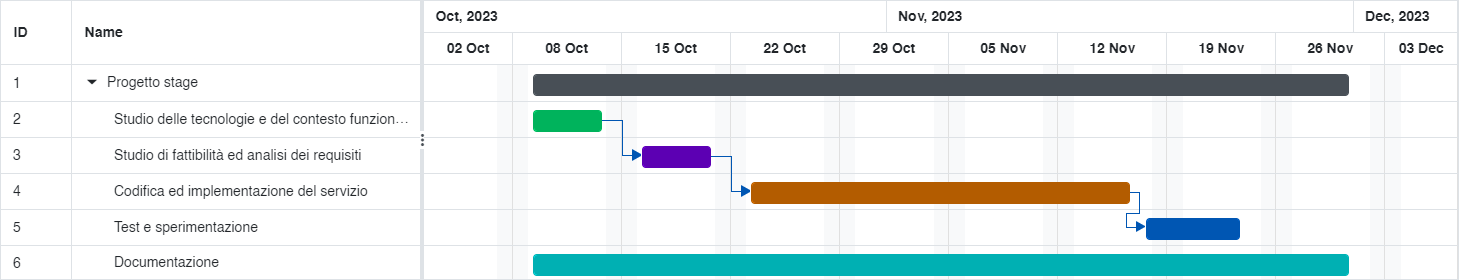
\includegraphics[width=\textwidth]{images/gantt.png}
    \caption{Diagramma di Gantt aggiornato con le attività svolte}
    \label{fig:gantt-finale}
\end{figure}

Di seguito vengono specificate le ore impiegate per ogni fase del progetto:
\begin{itemize}
    \item \textbf{Studio delle teconologie e del contesto funzionale:} per lo
          studio delle tecnologie da utilizzare sono state impiegate $40$ ore, in
          linea con il piano di lavoro iniziale;
    \item \textbf{Studio di fattibilità e analisi dei requisiti:} per effettuare
          l'analisi dei requisiti e lo studio di fattibilità sono state impiegate
          $40$ ore, in linea con quanto previsto dal piano di lavoro;
    \item \textbf{Codifica ed implementazione del servizio:} per la fase di
          codifica del servizio sono state impiegate $150$ ore, $30$ in più rispetto a
          quelle previste dal piano iniziale. Questo è dovuto al fatto che è stato
          speso molto più tempo nella fase di codifica della \emph{Proof of Concept},
          risultata poi fondamentale per lo sviluppo del servizio, in quanto ha
          permesso di accelerare di molto la fase di sviluppo del servizio in ambiente
          \emph{serverless};
    \item \textbf{Test e sperimentazione:} per la fase di test e sperimentazione
          sono state impiegate $34$ ore, $46$ in meno rispetto a quelle
          preventivate. Il motivo di tale discrepanza è dovuto a due aspetti: il primo
          riguarda i test, che sono stati scritti man mano che venivano sviluppate le
          funzionalità del servizio e ciò ha permesso di recuperare tempo che è stato
          impiegato nella fase di codifica per ottenere un codice più stabile. Il
          secondo aspetto riguarda la sperimentazione, che è stata fatta in maniera
          meno approfondita, preferendo la pulizia e la stabilità del codice scritto.
    \item \textbf{Documentazione:} per la fase di scrittura della documentazione
          sono state impiegate $40$ ore, in linea rispetto a quanto previsto nel piano
          di lavoro iniziale.
\end{itemize}

In totale sono state impiegate $304$ ore per il progetto di stage, $16$ ore in
meno rispetto alle $320$ previste inizialmente. Questo è da attribuirsi al fatto
che lo stage è terminato il $30/11/2023$, anziché il $01/12/2023$, poichè era
necessario che lo stage fosse terminato prima di tale data, al fine di poter
effettuare correttamente il
riconoscimento dei crediti dell'attività. Inoltre il giorno $01/11/2023$ era un
giorno di festività nazionale, che non è stato considerato nel piano di lavoro.